\section{Phương pháp luận}

\subsection{Thiết lập vấn đề}
Cho $D^s = \{(x^s, y^s)\}_{i=1}^{n_s}$ là một bộ dữ liệu đã thấy với các lớp $C^s$, trong đó mỗi hình ảnh $x \in \mathcal{X}$ có một nhãn tương ứng $y \in \mathcal{Y}^s$. Chúng ta cũng có một bộ dữ liệu chưa thấy $D^u = \{(x^u, y^u)\}_{j=1}^{n_u}$ với các lớp $C^u$. Theo thiết kế, $C^s$ và $C^u$ là rời rạc, đảm bảo $C^s \cap C^u = \emptyset$. Chúng ta ký hiệu thông tin ngữ nghĩa, tức là các thuộc tính, bằng $A = \{a_y\}_{y \in C^s \cup C^u}$ cho tất cả các lớp, trong khi chỉ có các lớp đã thấy là có sẵn để huấn luyện. Mục tiêu của chúng ta là huấn luyện một mô hình trên $D^s$ sao cho nó có thể nhận dạng chính xác các lớp trong $C^u$ tại thời điểm kiểm tra, mà không bao giờ thấy các ví dụ được gán nhãn cho $C^u$ trong quá trình huấn luyện.

\subsection{Động lực}
ZSL phụ thuộc vào việc căn chỉnh các đặc trưng thị giác với thông tin ngữ nghĩa. Tuy nhiên, thông tin không liên quan đến ngữ nghĩa trong không gian thị giác làm phức tạp sự căn chỉnh này. Nó tạo ra sự mơ hồ trong cách các thuộc tính ánh xạ đến các vùng hình ảnh có liên quan. Như thể hiện trong Hình \ref{fig:approaches}, các phương pháp hiện có loại bỏ thông tin không liên quan đến ngữ nghĩa trong (1) \textbf{không gian đặc trưng} (feature space), bằng cách xử lý sau các đặc trưng được trích xuất, hoặc (2) \textbf{không gian mô hình} (model space), bằng cách cắt bỏ các bản vá không liên quan trong các lớp khác nhau. Trong khi các chiến lược này phần nào ngăn chặn thông tin không liên quan đến ngữ nghĩa, chúng không loại bỏ hoàn toàn chúng. Do đó, nhiễu như vậy vẫn tồn tại trong các biểu diễn cuối
\begin{figure*}[t]
    \centering
    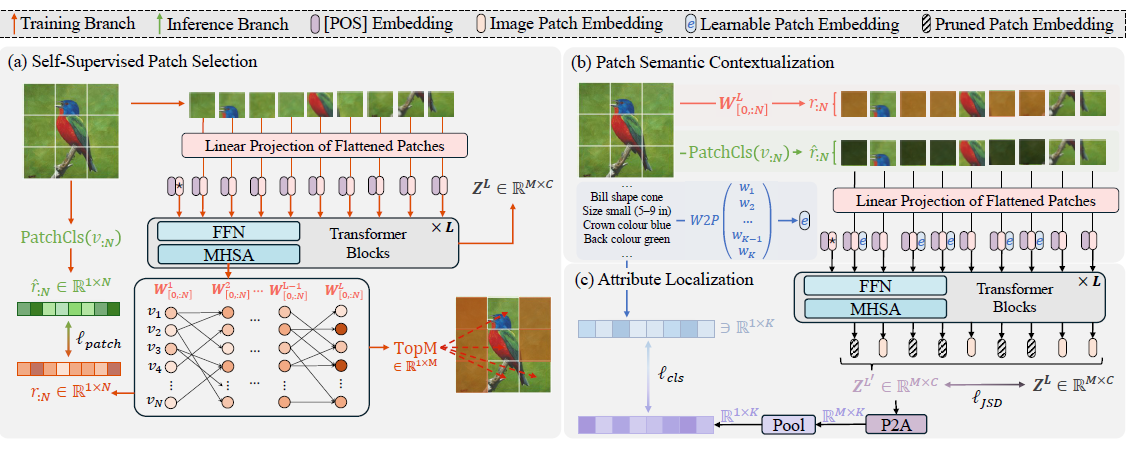
\includegraphics[width=\textwidth]{Image/Figure 2.PNG}
    \caption{Khung làm việc của SVIP được đề xuất của chúng tôi, bao gồm ba thành phần: (a) Lựa chọn bản vá Tự giám sát: chúng tôi tổng hợp các ma trận chú ý trong suốt các khối transformer để hướng dẫn việc huấn luyện bộ phân loại bản vá trong việc xác định các bản vá đầu vào không liên quan đến ngữ nghĩa. (b) Bối cảnh hóa Ngữ nghĩa Bản vá: chúng tôi áp dụng các nhúng bản vá có thể học được được khởi tạo bằng các nhúng từ thuộc tính để bối cảnh hóa các bản vá không liên quan đến ngữ nghĩa. (c) Cục bộ hóa Thuộc tính: chúng tôi cục bộ hóa các giá trị thuộc tính bằng các nhúng bản vá đầu ra cuối cùng, thay vì token lớp.}
    \label{fig:approaches}
\end{figure*}
cùng.

Ngược lại, như thể hiện trong Hình \ref{fig:framework}, chúng tôi đề xuất xác định và lọc các bản vá không liên quan đến ngữ nghĩa trong \textbf{không gian đầu vào} (input space), trước khi nó lan truyền vào mô hình. Sự can thiệp sớm này bảo tồn một biểu diễn sạch hơn, mạch lạc hơn về mặt ngữ nghĩa trong suốt quá trình trích xuất đặc trưng. Do đó, quy trình ZSL tiếp theo có thể tập trung vào các tương tác thị giác-ngữ nghĩa có ý nghĩa và cải thiện nhận dạng lớp chưa thấy.

\subsection{Lựa chọn bản vá Tự giám sát (Self-Supervised Patch Selection)}
Để khoanh vùng các bản vá không liên quan đến ngữ nghĩa, chúng tôi đề xuất một cơ chế Lựa chọn bản vá Tự giám sát (Self-Supervised Patch Selection - SSPS) huấn luyện một bộ phân loại nhị phân để dự đoán điểm ngữ nghĩa của các bản vá hình ảnh, sử dụng sự chú ý tổng hợp từ transformer làm giám sát.

\textbf{Revisiting ViT.} Chúng tôi phân chia một hình ảnh $x \in \mathbb{R}^{H \times W \times C}$ thành $N$ bản vá $\{p_1, \dots, p_N\}$. Mỗi bản vá sau đó được làm phẳng và chiếu tuyến tính thành một nhúng bản vá:
\begin{equation}
\{v_1, \dots, v_N\} = \text{PatchEmb}(\{p_1, \dots, p_N\}),
\end{equation}
chúng tôi thêm một token lớp có thể học $v_{cls}$ và thêm các nhúng vị trí $E_{pos}$ để tạo thành chuỗi bản vá ban đầu:
\begin{equation}
Z^0 = [v_{cls}, v_1, \dots, v_N] + E_{pos}.
\end{equation}
Chuỗi bản vá này đi qua $L$ khối transformer:
\begin{equation}
Z^l = \text{TransformerBlock}^l(Z^{l-1}), l=1, \dots, L.
\end{equation}
tạo ra các đầu ra cuối cùng $Z^L = [z_{cls}, z_1, \dots, z_N]$. Ở đây, token lớp $z_{cls}$ được lấy làm biểu diễn toàn cục.

\textbf{Giám sát bản vá thông qua Tổng hợp Ma trận Chú ý.} Để ước tính điểm ngữ nghĩa của mỗi bản vá, chúng tôi thu thập các điểm chú ý từ các khối tự chú ý đa đầu (MHSA). Cho $T^l \in \mathbb{R}^{(N+1) \times (N+1)}$ là ma trận chú ý trong khối transformer thứ $l$ được tổng hợp trên tất cả các đầu chú ý. Chúng tôi tổng hợp các điểm chú ý này qua các lớp:
\begin{equation}
W^l = W^{l-1} + W^{l-1} \times T^l, l=1, \dots, L,
\end{equation}
trong đó $W^1 = T^1$. Ma trận tổng hợp $W^L$ cung cấp một cái nhìn toàn cục về tầm quan trọng của bản vá. Chúng tôi tiếp tục lấy hàng tương ứng với token lớp (chỉ số 0) để cung cấp điểm của mỗi bản vá: $r_i = W^L_{[0, i]}$, có thể dùng làm nhãn giả của các điểm ngữ nghĩa.
Sau đó, chúng tôi giới thiệu một bộ phân loại bản vá phụ để dự đoán điểm ngữ nghĩa của mỗi nhúng bản vá:
\begin{equation}
\hat{r}_i = \text{PatchCls}(v_i), i=1, \dots, N.
\end{equation}
Việc căn chỉnh $\hat{r}_i$ với $r_i$ có nguồn gốc từ sự chú ý cho phép mô hình học sự phân biệt bản vá ngữ nghĩa chi tiết với một mất mát entropy chéo nhị phân:
\begin{equation}
\mathcal{L}_{patch} = -\frac{1}{N} \sum_{i=1}^{N} [r_i \log(\hat{r}_i) + (1-r_i)\log(1-\hat{r}_i)].
\end{equation}
Thiết kế này được thúc đẩy bởi tính chất động của các điểm chú ý qua các lớp transformer. Như thể hiện trong Hình \ref{fig:attention_visualization}, chúng tôi trực quan hóa điểm chú ý của 49 bản vá trên 12 lớp transformer. Tầm quan trọng của các bản vá này không nhất quán qua các lớp khác nhau. Do đó, việc dựa vào một số lớp nhất định để xác định các bản vá không liên quan đến ngữ nghĩa có thể dẫn đến phân loại sai. Trong SSPS, chúng tôi tạo ra các nhãn giả mạnh mẽ hơn bằng cách tổng hợp các điểm chú ý trên tất cả các lớp.

\begin{figure}[t]
    \centering
    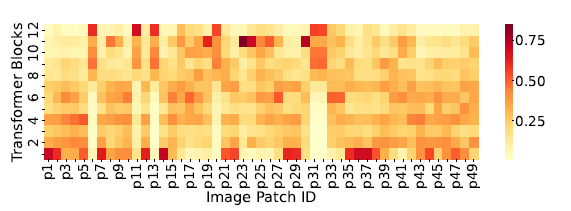
\includegraphics[width=0.9\columnwidth]{Image/Figure 3.PNG}
    \caption{Một trực quan hóa về trọng số chú ý của bản vá trên tất cả các lớp tự chú ý trong ViT.}
    \label{fig:attention_visualization_2}
\end{figure}

\subsection{Bối cảnh hóa Ngữ nghĩa Bản vá (Patch Semantic Contextualization)}
Mặc dù việc loại bỏ các bản vá không liên quan đến ngữ nghĩa có thể chỉ bảo tồn các bản vá thông tin, nó có thể phá vỡ cấu trúc đối tượng. Thay vào đó, chúng tôi đề xuất Bối cảnh hóa Ngữ nghĩa Bản vá (Patch Semantic Contextualization - PSC) để bối cảnh hóa các bản vá này với thông tin cấp thuộc tính, biến đổi các nhúng của chúng để căn chỉnh tốt hơn với ngữ nghĩa.

\textbf{Nhúng bản vá có thể học.} Chúng tôi định nghĩa một nhúng bản vá có thể học $e$ được khởi tạo từ các véc-tơ từ \cite{39}. Cho $\{w_1, \dots, w_K\}$ là các nhúng từ cho $K$ thuộc tính (ví dụ: màu sắc, hình dạng). Chúng được tổng hợp thông qua một lớp chiếu Word-to-Patch (W2P):
\begin{equation}
e = \text{W2P}(w_1, \dots, w_K).
\end{equation}
Tiếp theo, chúng tôi xác định các bản vá có điểm dự đoán $\hat{r}_i$ vượt quá một ngưỡng hoặc xếp hạng trong top $M$:
\begin{equation}
S_M = \text{TopM}_{i \in \{1, \dots, N\}} \{\hat{r}_i, M\}.
\end{equation}
Sau đó, chúng tôi đưa $e$ vào mỗi bản vá được chọn như tiêm các nhúng vị trí:
\begin{equation}
Z^{0'} = [v_{cls}, v'_1, \dots, v'_N] + E_{pos}, \quad v'_i = 
\begin{cases}
    v_i + e, & \text{nếu } i \in S_M \\
    v_i, & \text{khác}.
\end{cases}
\end{equation}
Bởi vì các nhúng bản vá được cập nhật $v'_i$ mang thông tin ngữ nghĩa cấp thuộc tính trong không gian đầu vào, điều này có thể tăng cường tương tác thị giác-ngữ nghĩa trong suốt các khối transformer.

\subsection{Cục bộ hóa Thuộc tính (Attribute Localization)}
Mặc dù token lớp cuối cùng $z_{cls}$ có thể nắm bắt biểu diễn toàn cục, các bản vá liên quan đến ngữ nghĩa có thể giúp cục bộ hóa các thuộc tính. Cho $Z^{L'} = \{z'_i | i \in S_M\}$ là các biểu diễn cuối cùng của top $M$ bản vá liên quan đến ngữ nghĩa. Chúng tôi học một hàm chiếu Patch-to-Attribute (P2A) để ánh xạ các nhúng bản vá $Z^{L'} \in \mathbb{R}^{M \times C}$ vào không gian thuộc tính: $\hat{A} = \text{P2A}(Z^{L'}) \in \mathbb{R}^{M \times K}$, trong đó $K$ là số lượng thuộc tính mô tả một danh mục. Một hoạt động gộp tối đa (max pooling) sau đó được áp dụng trên các nhúng thuộc tính bản vá này:
\begin{equation}
\hat{a} = \text{MaxPool}(\hat{A}),
\end{equation}
xác định bản vá phù hợp nhất cho mỗi thuộc tính. Do đó, mô hình học cách tập trung khi dự đoán một giá trị thuộc tính. Xác suất phân loại tuân theo một SoftMax tiêu chuẩn trên các điểm tương đồng cosine:
\begin{equation}
p(y|Z^0) = \frac{\exp(\sigma \cdot \cos(\hat{a}, a_y))}{\sum_{\tilde{y} \in \mathcal{Y}^s} \exp(\sigma \cdot \cos(\hat{a}, a_{\tilde{y}}))},
\end{equation}
trong đó $a_y$ là véc-tơ thuộc tính của một lớp đã thấy $y$ và $\sigma$ là nhiệt độ để điều chỉnh các điểm tương đồng cosine.

\subsection{Tối ưu hóa và Suy luận Mô hình}
\textbf{Tối ưu hóa.} Chúng tôi truyền mỗi mẫu qua các khối transformer hai lần: một lần với các bản vá gốc $Z^0$ và một lần với các bản vá được bối cảnh hóa $Z^{0'}$. Do đó, mất mát phân loại của chúng tôi tổng hợp cả hai dự đoán:
\begin{equation}
\mathcal{L}_{cls} = -\log p(y|Z^0) - \log p(y|Z^{0'}).
\end{equation}
Để ổn định việc huấn luyện cho các bản vá được bối cảnh hóa, chúng tôi áp dụng phân kỳ Jensen-Shannon (Jensen-Shannon divergence) giữa hai phân phối đầu ra:
\begin{equation}
\mathcal{L}_{JSD} = \frac{1}{2} D_{KL}(p(y|Z^0) \parallel \bar{p}) + \frac{1}{2} D_{KL}(p(y|Z^{0'}) \parallel \bar{p})
\end{equation}
với $\bar{p} = \frac{1}{2}(p(y|Z^0) + p(y|Z^{0'}))$.
Nhìn chung, mục tiêu huấn luyện được định nghĩa là:
\begin{equation}
\mathcal{L}_{overall} = \mathcal{L}_{cls} + \lambda_1 \mathcal{L}_{JSD} + \lambda_2 \mathcal{L}_{patch},
\end{equation}
trong đó $\lambda_1$ và $\lambda_2$ là các hệ số mất mát. Toàn bộ quá trình huấn luyện được minh họa trong Thuật toán 1.

\textbf{Suy luận Zero-Shot.} Đầu tiên, chúng tôi phân vùng một hình ảnh thử nghiệm thành nhiều bản vá và chiếu chúng thành các nhúng bản vá tương ứng bằng Eq. (1). Sau đó, chúng tôi xác định các bản vá không liên quan đến ngữ nghĩa bằng bộ phân loại bản vá đã học bằng Eq. (5). Trong khi tất cả các nhúng bản vá được áp dụng với các nhúng vị trí, chỉ những bản vá không liên quan đến ngữ nghĩa mới được áp dụng với các nhúng bản vá ngữ nghĩa đã học như trong Eq. (9). Các nhúng bản vá này được đưa vào các khối transformer để cục bộ hóa thuộc tính hơn nữa. Cuối cùng, chúng tôi suy ra nhãn lớp chưa thấy được dự đoán bằng Eq. (11).
